\documentclass[UTF8]{ctexart}
\ctexset { section = { format={\Large \bfseries } } }
\pagestyle{plain}
\setlength{\parindent}{0pt}
\usepackage{float}
\usepackage{amsmath}
\usepackage{amssymb}
\usepackage{listings}
\usepackage{graphicx}%插入图片宏包
\usepackage{xcolor}
\usepackage{geometry}
\geometry{a4paper,scale=0.8}
\usepackage{caption}
\usepackage{subcaption}
\usepackage[colorlinks=true, linkcolor=blue, citecolor=blue, urlcolor=blue]{hyperref}
\captionsetup[figure]{name={Figure}}
\captionsetup[table]{name={Table}}
\definecolor{Rhodamine}{RGB}{227,11,92}


\lstset{
language=Python, % 设置语言
basicstyle=\ttfamily\small, % 设置字体族
breaklines=true, % 自动换行
keywordstyle=\bfseries\color{blue}, % 设置关键字为粗体,
morekeywords={}, % 设置更多的关键字,用逗号分隔
emph={self}, % 指定强调词,如果有多个,用逗号隔开
emphstyle=\bfseries\color{Rhodamine}, % 强调词样式设置
commentstyle=\color{black!50!white}, % 设置注释样式,斜体,浅灰色
stringstyle=\bfseries\color{red!90!black}, % 设置字符串样式
columns=flexible,
numbers=left, % 显示行号在左边
numbersep=2em, % 设置行号的具体位置
numberstyle=\footnotesize, % 缩小行号
frame=single, % 边框
framesep=1em, % 设置代码与边框的距离
showstringspaces=false
}

\title{\textbf{Image Processing Homework 7}}
\author{吴嘉骜 21307130203}
\date{\today}

\begin{document}

\maketitle

{\large \textbf{Image Spatial Transformation}}

Implement: (1) A local affine transformation (or FFD-based deformation algorithm) for spatial transformation, 
(2) and applying this spatial transformation in a backward image transformation process to achieve the image transformation from Image $A$ to Image $B$. 
The basic algorithmic content of the assignment can refer to the classroom teaching and courseware.

Note: You may refer to other academic materials to improve the effect (optional), but you cannot solely use other algorithms without implementing the two basic requirements of the topic.

\textbf{Solution}:\\
In this problem, I chose the local affine transformation to implement the spatial transformation.
The main work can be divided into two parts: the local affine transformation, and the backward image transformation process.

\section{Local Affine Transformation}
In this context, we consider a source image and a destination image, and we want to transform the former to the later by a local affine transformation.
The main steps are as follows:\\

1. Calculate the transformation matrix $T$ for each control point.

\begin{lstlisting}
def get_T(x_s, y_s, x_d, y_d):
    '''
    get translation matrix T (3D, for each point)
    :param x_s, y_s: source points' coordinates, each is an array.
    :param x_d, y_d: destination points' coordinates, each is an array.
    '''
    num = np.array(x_s).shape[0]
    T = np.zeros((num, 3, 3))
    for i in range(num):
        T[i] = np.array(
            [[1, 0, 0], [0, 1, 0], [x_d[i] - x_s[i], y_d[i] - y_s[i], 1]])
    return T
\end{lstlisting}

To simplify the problem and save processing time, I only consider point control, and $T$ is a translation matrix.
For each control point $(x_s, y_s)$, we have the corresponding point $(x_d, y_d)$, and $T$ is a $3\times 3$ matrix satisfying $[x_d, y_d, 1] = [x_s, y_s, 1]T$.
Above we have $n$ control points, so we have $n$ $T$ matrices, which are stored in a $n\times 3\times 3$ matrix.\\

In fact, for region control, we can solve a linear system to get the $T$ matrix, which is usually a least square problem.
If we have more explicit correspondences, we can also generate $T$ by the definition of affine transformation.\\

2. For each pixel in the source image, calculate the transformed coordinates by the weighted average formula.\\

First, we need to calculate the weight matrix $W$ for each pixel, which depends on the distance between the pixel and each control point.
The weight calculation takes into account the influence of each control point based on its distance to the pixel.
The weights are inversely proportional to the distance, raised to a power $e$.\\

\begin{lstlisting}
def get_dist(u, v, x, y):
    dist = np.sqrt((u - x) ** 2 + (v - y) ** 2)
    eps = 1e-8
    if dist < eps:  # avoid zero division
        return eps
    else:
        return dist

def get_weight(u, v, x_c, y_c, e):
    '''
    get weight matrix (an array, weights from point(x,y) to all control points)
    :param u, v: point in consideration
    :param x_c, y_c: control points' coordinates, each is an array.
    :param e: exponent in weight calculation
    '''
    num = np.array(x_c).shape[0]
    weight = np.zeros((num, 1))
    for i in range(num):
        x, y = x_c[i], y_c[i]
        dist = get_dist(u, v, x, y)
        weight[i] = dist ** (-e)
    weight = weight / np.sum(weight)
    return weight
\end{lstlisting}

After calculating the weights, we determine the transformed coordinates for each pixel in the destination image.
This is achieved by taking the weighted average of the potential transformed coordinates based on each control point's transformation matrix $T$.
The transformed coordinates are computed by multiplying the source point (in homogeneous coordinates) by each control point's transformation matrix.
The final transformed coordinates of the pixel are the sum of these weighted coordinates.

Note that we do not distinguish control points (whose transformed coordinates are known ahead and should not be calculated by the weighted average formula) and other points
in the source image. The reason is that we specify the distance of a point to itself to be $10^{-8}$ so the weight along with its own transformed coordinates
is far larger than the weights of other points. By normalizing the weights, we can get almost the same result as if we directly use the control points' destination coordinates.\\

\begin{lstlisting}
def get_transcorr(u, v, x_c, y_c, T, e):
    '''
    get transformed coordinates
    :param u, v: point in consideration
    :param x_c, y_c: control points' coordinates, each is an array.
    :param T: transformation matrix
    :param e: exponent in weight calculation
    '''
    num = np.array(x_c).shape[0]
    w = get_weight(u, v, x_c, y_c, e)
    des = np.zeros((num, 2))  # destination points for every T[i] (2D)
    for i in range(num):
        s = np.array([u, v, 1])  # source point (homogeneous coordinates)
        d = np.matmul(s, T[i])  # destination point (homogeneous coordinates)
        x, y, _ = d
        des[i] = np.array([x, y])
    tmp = w * des
    new_u = np.sum(tmp[:, 0])
    new_v = np.sum(tmp[:, 1])
    return new_u, new_v
\end{lstlisting}


The full codes from \texttt{loc\_affine.py} in this section are listed in \hyperlink{code1}{Appendix A}.


\section{Backward Image Transformation}

The backward image transformation process is as follows:\\
1. For each pixel in the destination image, calculate the transformed coordinates in the source image by the local affine transformation.\\
2. Perform bilinear interpolation to get the pixel intensity value in the destination image.\\

The core codes in the above steps are shown as follows:\\
\begin{lstlisting}
import loc_affine as af

def back_trans(img, x_d, y_d, x_s, y_s, e):
    '''
    Backward transformation
    :param img: source image
    :param x_d, y_d: destination points' coordinates, each is an array.
    :param x_s, y_s: source points' coordinates, each is an array.
    :param e: exponent in weight calculation
    '''
    new_img = np.zeros_like(img)  # destination image
    h, w, _ = img.shape
    # get affine transformation matrix T
    T = af.get_T(x_d, y_d, x_s, y_s)
    for i in range(h):
        for j in range(w):
            # get new coordinates
            new_i, new_j = af.get_transcorr(i, j, x_d, y_d, T, e)
            # bilinear interpolation
            new_img[i, j] = bilin(img, new_i, new_j)
    
    return new_img
\end{lstlisting}

The full codes from part of \texttt{backtrans.py} in this section are listed in \hyperlink{code2}{Appendix B}.

\section{Experiment Results}
To test the performance of the algorithm, I utilize \texttt{matplotlib} for interactive selection of control points.
The setup involves simultaneously displaying images of source and destination.
The user then can alternately click on control points in the two images under instructions, denoting correspondences between the two images.
Closing the window will trigger the algorithm to run, and the transformed image will be displayed.

The full codes from part of \texttt{backtrans.py} in this section are listed in \hyperlink{code3}{Appendix C}.\\

We experiment with a human face (courtesy of President Putin) and a mandrill. We select 4 control points for each eye,
3 for the nose and 3 for the mouth. The exponent $e$ in weight calculation is set to be 2 and 3 respectively.
Results are shown in Figure \ref{fig:aff}.\\
\newpage
\begin{figure}[htbp]
    \centering
    \begin{subfigure}{0.3\textwidth}
        \centering
        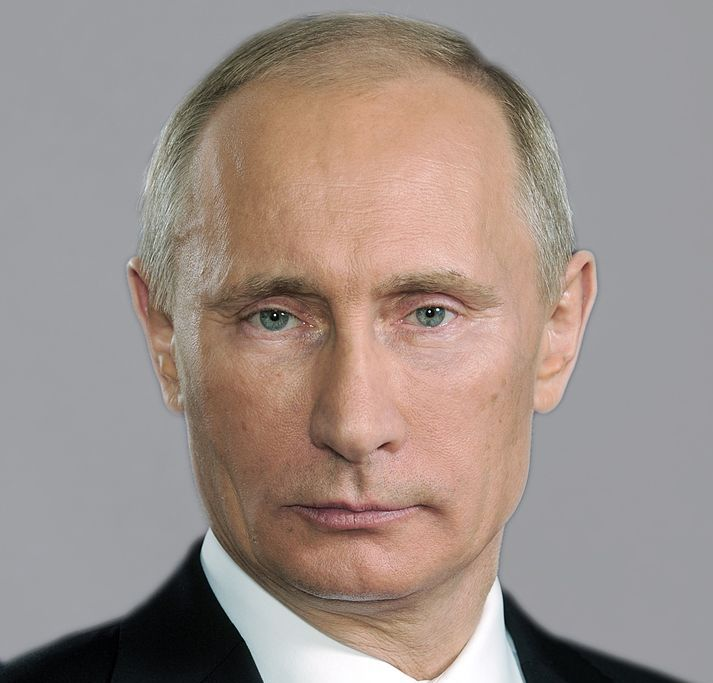
\includegraphics[width=\linewidth]{Putin.jpg}
        \caption{Original human image}
    \end{subfigure}%
    \hfill
    \begin{subfigure}{0.3\textwidth}
        \centering
        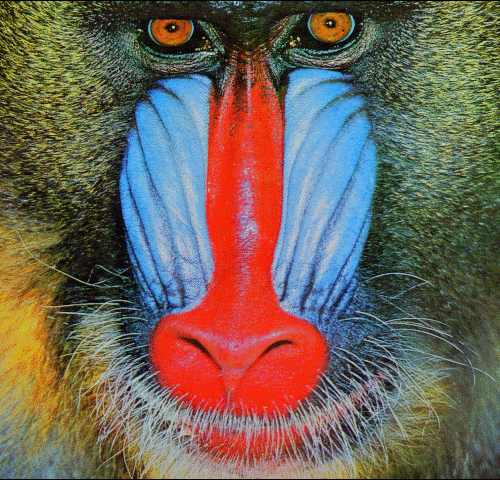
\includegraphics[width=\linewidth]{mandrill.png}
        \caption{Reference mandrill image}
    \end{subfigure}%
    \hfill
    \begin{subfigure}{0.3\textwidth}
        \centering
        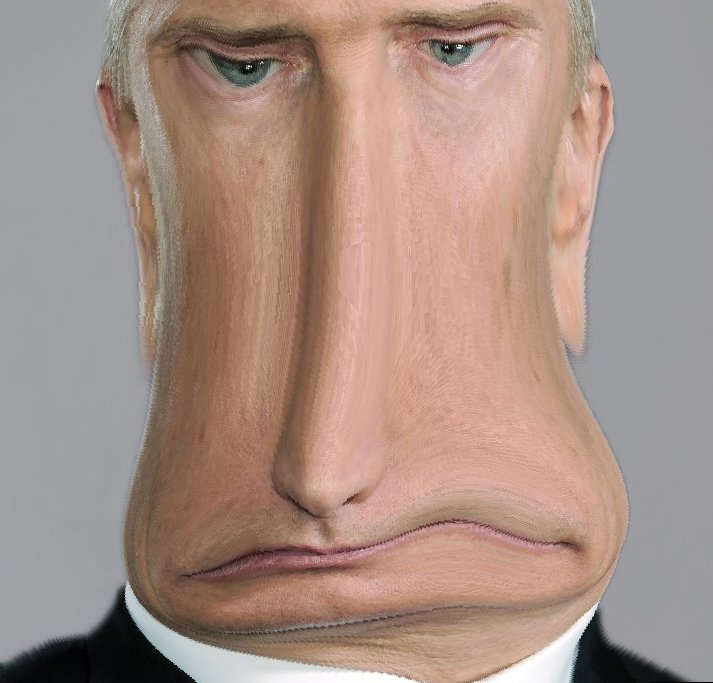
\includegraphics[width=\linewidth]{putinreg2.png}
        \caption{Transformed image, $e=2$}
    \end{subfigure}%
    \vspace{0.5cm}
    \begin{subfigure}{0.65\textwidth}
        \centering
        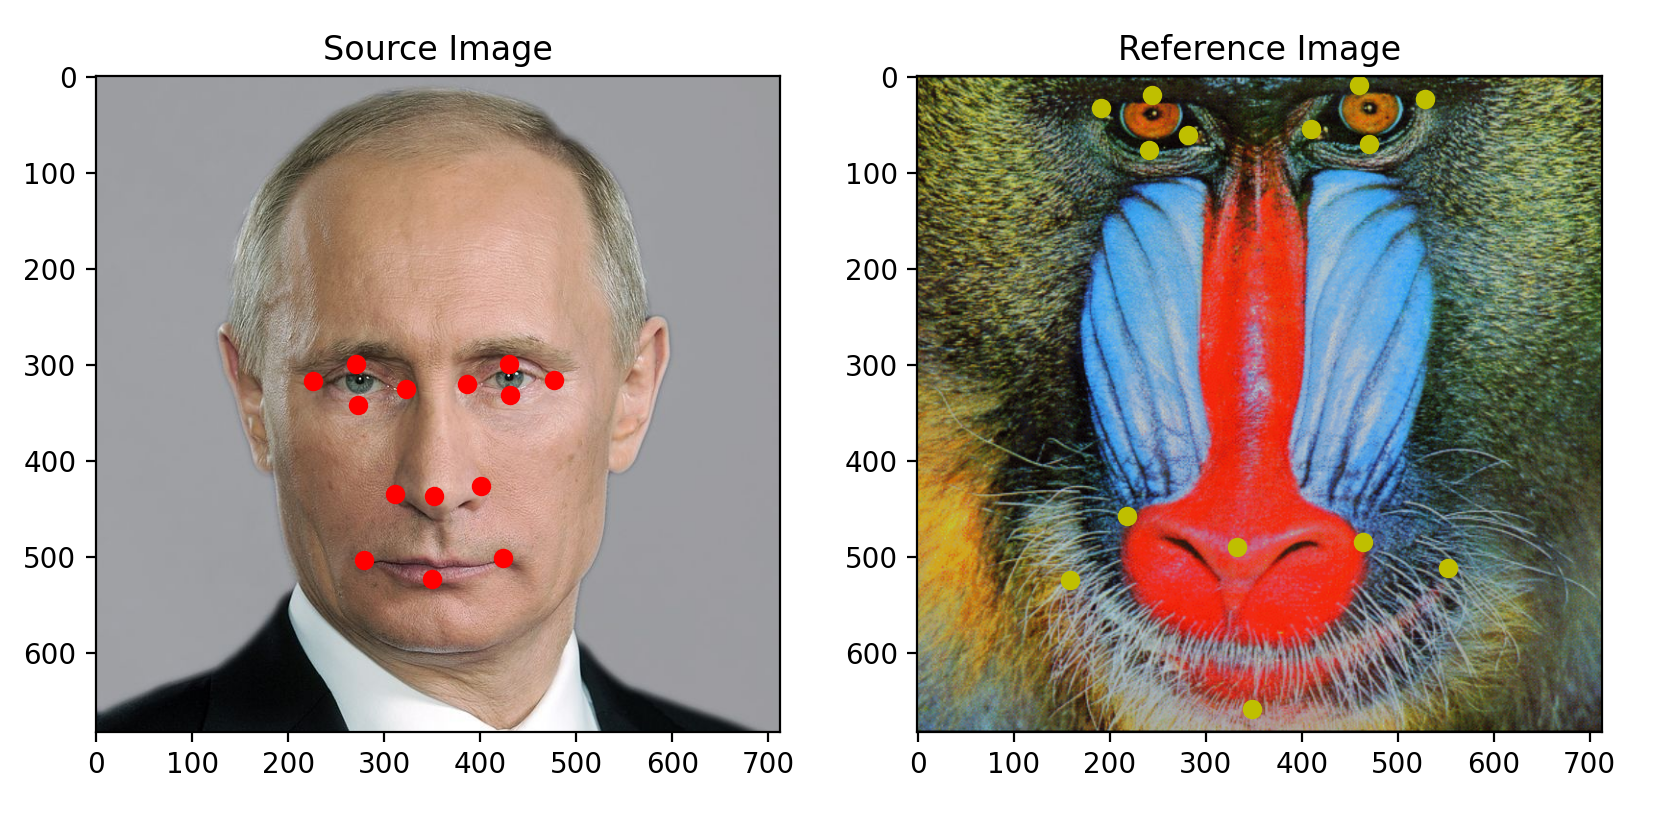
\includegraphics[width=\linewidth]{selection.png}
        \caption{Selection of control points}
    \end{subfigure}
    \hfill
    \begin{subfigure}{0.3\textwidth}
        \centering
        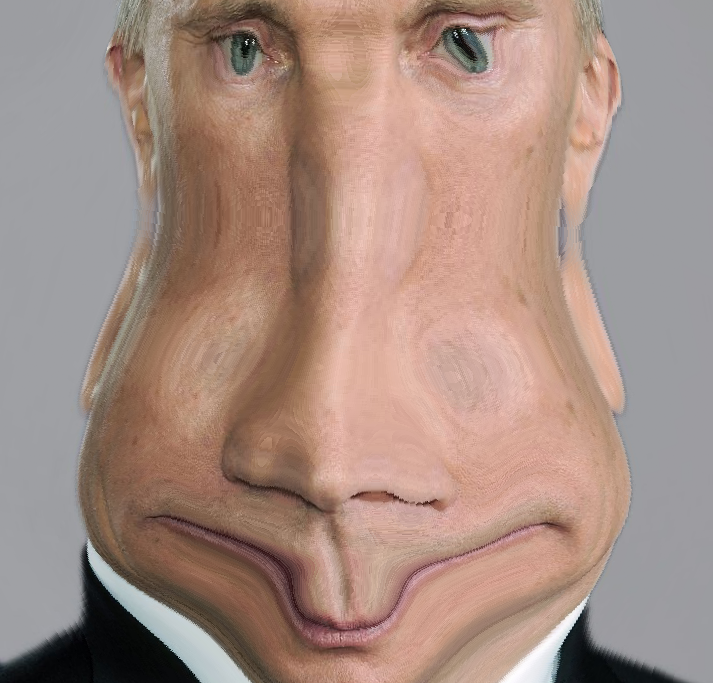
\includegraphics[width=\linewidth]{putinreg3.png}
        \caption{Transformed image, $e=3$}
    \end{subfigure}%
    \caption{Backward local affine transformation}
    \label{fig:aff}
\end{figure}

We can see that the transformed image is similar to the reference image, but the result is not very satisfactory.
The reason is that the translation transformation is not only not very flexible, but sensitive to the selection of control points.
If we select more control points, the result will be awkward and disturbing as there appear too many ``holes'' in the transformed image.
And the position of the control points also matters. If we select the control points in the eyes too close to the center,
the transformed image will be very strange since the eyes are distorted.\\
Comparing the results with different $e$, we can see that the transformed image with $e=3$ is more similar to the reference image, but
with some imaginary features presented. This is probably because the weights of control points are more concentrated on the nearest control points.\\
To further improve the result, we should consider region control together with point control, and more complicated affine transformation models.
We can also use other algorithms, such as thin-plate spline and FFD. 


\newpage
\appendix
\hypertarget{code1}{\section{Code for local affine transformation}}
\begin{lstlisting}
import numpy as np


# point control: translation
def get_T(x_s, y_s, x_d, y_d):
    '''
    get translation matrix T (3D, for each point)
    :param x_s, y_s: source points' coordinates, each is an array.
    :param x_d, y_d: destination points' coordinates, each is an array.
    '''
    num = np.array(x_s).shape[0]
    T = np.zeros((num, 3, 3))
    for i in range(num):
        T[i] = np.array(
            [[1, 0, 0], [0, 1, 0], [x_d[i] - x_s[i], y_d[i] - y_s[i], 1]])
    return T

def get_dist(u, v, x, y):
    dist = np.sqrt((u - x) ** 2 + (v - y) ** 2)
    eps = 1e-8
    if dist < eps:  # avoid zero division
        return eps
    else:
        return dist

def get_weight(u, v, x_c, y_c, e):
    '''
    get weight matrix (an array, weights from point(x,y) to all control points)
    :param u, v: point in consideration
    :param x_c, y_c: control points' coordinates, each is an array.
    :param e: exponent in weight calculation
    '''
    num = np.array(x_c).shape[0]
    weight = np.zeros((num, 1))
    for i in range(num):
        x, y = x_c[i], y_c[i]
        dist = get_dist(u, v, x, y)
        weight[i] = dist ** (-e)
    weight = weight / np.sum(weight)
    return weight

def get_transcorr(u, v, x_c, y_c, T, e):
    '''
    get transformed coordinates
    :param u, v: point in consideration
    :param x_c, y_c: control points' coordinates, each is an array.
    :param T: transformation matrix
    :param e: exponent in weight calculation
    '''
    num = np.array(x_c).shape[0]
    w = get_weight(u, v, x_c, y_c, e)
    des = np.zeros((num, 2))  # destination points for every T[i] (2D)
    for i in range(num):
        s = np.array([u, v, 1])  # source point (homogeneous coordinates)
        d = np.matmul(s, T[i])  # destination point (homogeneous coordinates)
        x, y, _ = d
        des[i] = np.array([x, y])
    tmp = w * des
    new_u = np.sum(tmp[:, 0])
    new_v = np.sum(tmp[:, 1])
    return new_u, new_v
\end{lstlisting}

\hypertarget{code2}{\section{Code for backward transformation}}
\begin{lstlisting}
from PIL import Image
import numpy as np
import matplotlib.pyplot as plt
import cv2
import loc_affine as af

def save_img(img, save_path):
    img = Image.fromarray(img)
    img.save(save_path)

def bilin(image, i, j):
    """
    Perform bilinear interpolation for a given point.

    :param image: Input color image as a NumPy array with shape (rows, cols, 3).
    :param i, j: The row, column coordinates of the point for interpolation.
    :return: Interpolated 3-channel value at point (i, j).
    """
    rows, cols, _ = image.shape
    # Calculate the integer parts of i and j
    up = int(np.floor(i))
    down = int(np.ceil(i))
    left = int(np.floor(j))
    right = int(np.ceil(j))
    # Return a zero vector for out-of-bound coordinates
    if up < 0 or left < 0 or down >= rows or right >= cols:
        return np.zeros(3)
    # Calculate the differences
    di = i - up
    dj = j - left
    # Perform bilinear interpolation for each channel
    new_value = np.zeros(3)
    for c in range(3):  # Loop over each color channel
        new_value[c] = (di * dj * image[up, left, c] +
                                    di * (1 - dj) * image[up, right, c] +
                                    (1 - di) * dj * image[down, left, c] +
                                    (1 - di) * (1 - dj) * image[down, right, c])
    return new_value

def back_trans(img, x_d, y_d, x_s, y_s, e):
    '''
    Backward transformation
    :param img: source image
    :param x_d, y_d: destination points' coordinates, each is an array.
    :param x_s, y_s: source points' coordinates, each is an array.
    :param e: exponent in weight calculation
    '''
    new_img = np.zeros_like(img)  # destination image
    h, w, _ = img.shape
    # get affine transformation matrix T
    T = af.get_T(x_d, y_d, x_s, y_s)
    for i in range(h):
        for j in range(w):
            # get new coordinates
            new_i, new_j = af.get_transcorr(i, j, x_d, y_d, T, e)
            # bilinear interpolation
            new_img[i, j] = bilin(img, new_i, new_j)
    
    return new_img
\end{lstlisting}

\hypertarget{code3}{\section{Code for interactive selection of control points}}
\begin{lstlisting}
class ControlPointsSelector:
    def __init__(self, img1, img2):
        self.fig, self.axs = plt.subplots(1, 2)
        self.axs[0].imshow(img1)
        self.axs[1].imshow(img2)
        self.axs[0].set_title('Source Image')
        self.axs[1].set_title('Reference Image')

        self.x_s, self.y_s = [], []
        self.x_d, self.y_d = [], []
        self.selecting_source = True  # Start by selecting from the left image

        self.status_text = self.fig.text(0.05, 0.95, 'Select a point on the left image.',
                                         transform=self.fig.transFigure,
                                         ha="left", va="top", color="black")
        self.cid = self.fig.canvas.mpl_connect(
            'button_press_event', self.onclick)

    def onclick(self, event):
        ax_index = 0 if self.selecting_source else 1
        if event.inaxes == self.axs[ax_index]:
            x, y = round(event.xdata), round(event.ydata)

            if self.selecting_source:
                self.x_s.append(x)
                self.y_s.append(y)
                self.axs[0].plot(x, y, 'ro')  # Add red dot
            else:
                self.x_d.append(x)
                self.y_d.append(y)
                self.axs[1].plot(x, y, 'yo')  # Add yellow dot

            # Update the status text
            if self.selecting_source:
                self.status_text.set_text('Select a point on the right image.')
                self.status_text.set_color('black')
            else:
                self.status_text.set_text('Select a point on the left image.')
                self.status_text.set_color('black')

            # Update the canvas
            self.fig.canvas.draw()

            # Toggle between source and destination
            self.selecting_source = not self.selecting_source

    def show(self):
        plt.show()
\end{lstlisting}
\end{document}